\chapter{実験結果と考察}
本章では,前章で述べた提案手法の有効性を検証するために行ったシミュレーション実験の結果について報告する。
また,各実験結果に基づき,提案手法が持つ課題やその改善の可能性について考察する.

\section{避難者探索タスク実験}
\subsection{モデル学習結果}
\subsection{実験結果}
\subsection{実験結果の考察}

\section{避難所誘導タスクの結果}
\subsection{モデル学習結果}
図\ref{fig:YokosukaModel-Result}~は各都市におけるマルチエージェントモデルの学習過程のグラフである.エントロピーの推移,グループ報酬の推移,ポリシー関数の平均損失
,価値関数の平均損失のグラフを示す.
\begin{figure}[H]
  \centering
  % 1枚目の画像
  \begin{subfigure}{0.45\textwidth}
      \centering
      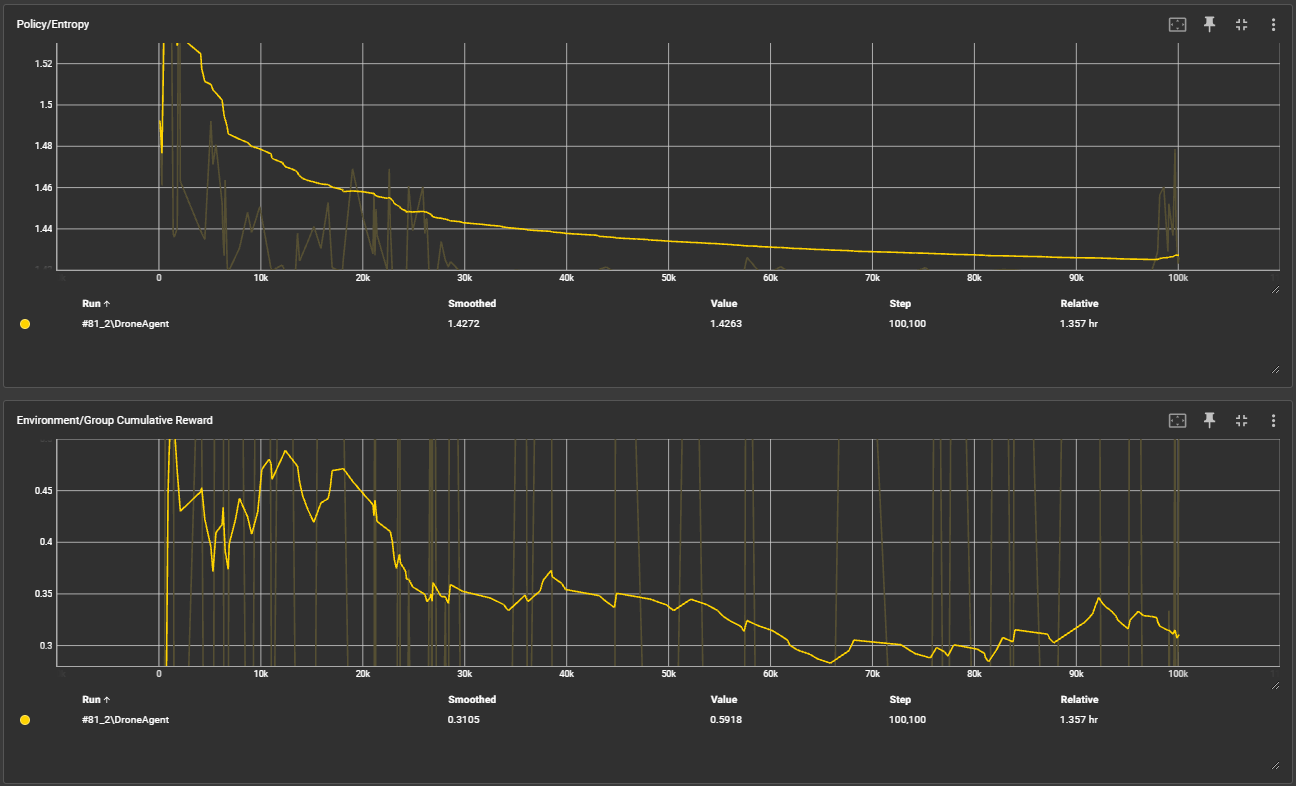
\includegraphics[width=\textwidth]{Figures/YokosukaModel-Result.png}
      \caption{横須賀市環境での訓練結果}
      \label{fig:YokosukaModel-Result}
  \end{subfigure}
  % 2枚目の画像
  \begin{subfigure}{0.45\textwidth}
      \centering
      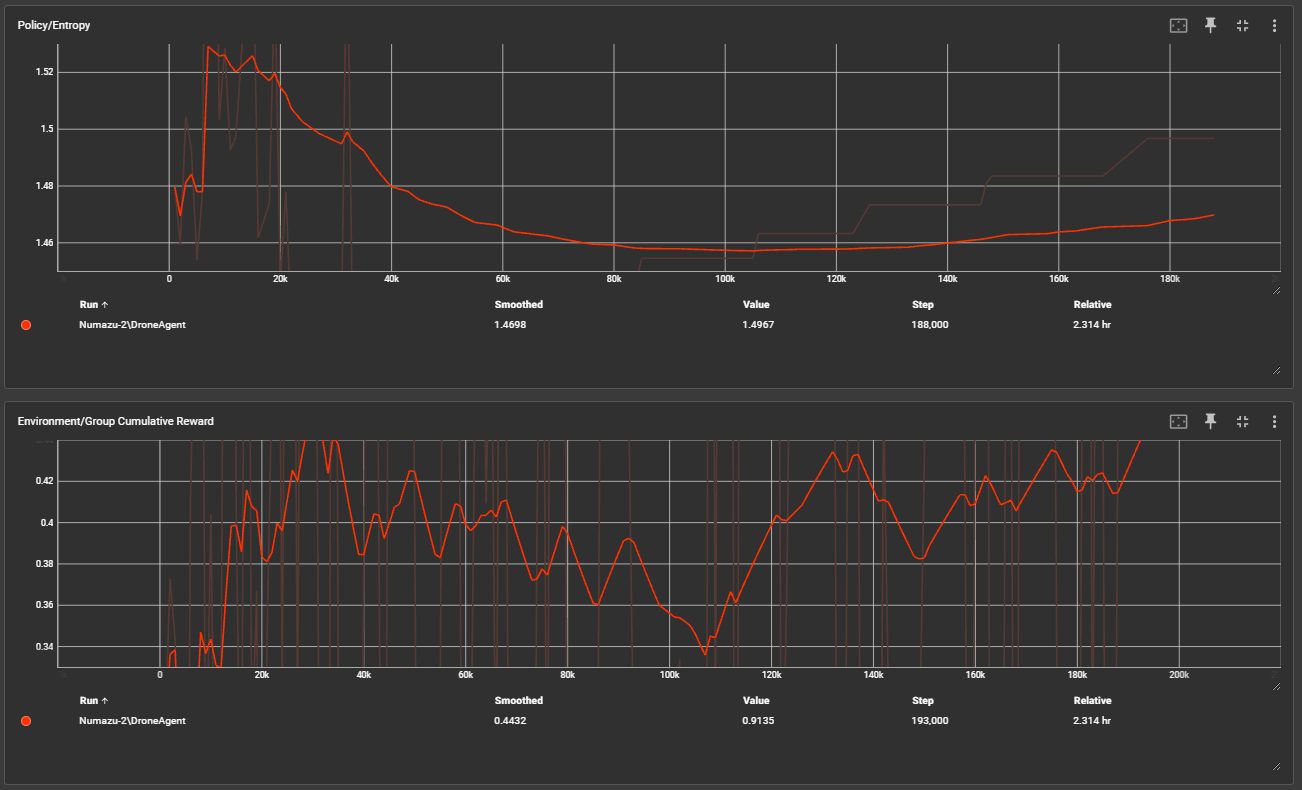
\includegraphics[width=\textwidth]{Figures/NumazuModel-Result.png}
      \caption{沼津市環境での訓練結果}
      \label{fig:NumazuModel-Result}
  \end{subfigure}
  \caption{両都市モデルでのエントロピー(上)とグループ報酬(下)の推移}
  \label{fig:Model-Result1}
\end{figure}
\begin{figure}[H]
  \centering
  % 1枚目の画像
  \begin{subfigure}{0.45\textwidth}
      \centering
      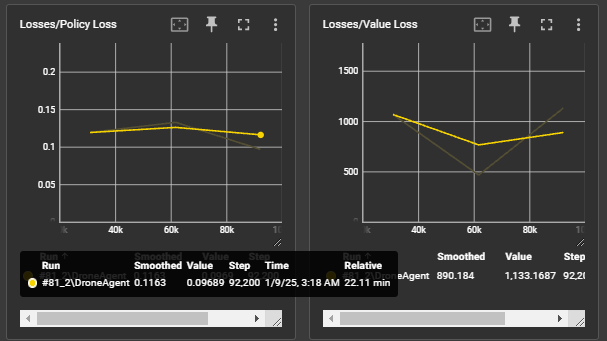
\includegraphics[width=\textwidth]{Figures/Yokosuka-Loss.png}
      \caption{横須賀市環境での訓練結果}
      \label{fig:YokosukaModel-Result2}
  \end{subfigure}
  % 2枚目の画像
  \begin{subfigure}{0.45\textwidth}
      \centering
      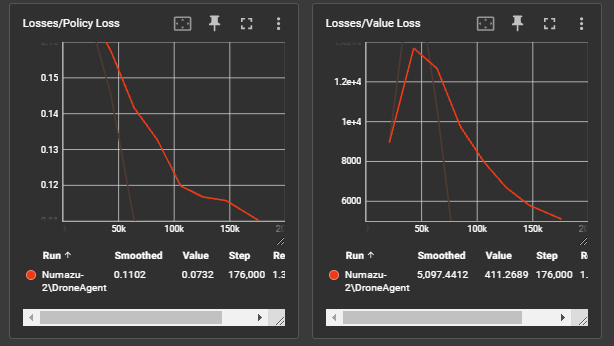
\includegraphics[width=\textwidth]{Figures/Numazu-Loss.png}
      \caption{沼津市環境での訓練結果}
      \label{fig:NumazuModel-Result2}
  \end{subfigure}
  \caption{ポリシー関数の平均損失(左)と価値関数の平均損失(右)}
  \label{fig:Model-Result-Errors}
\end{figure}
まずエントロピーの結果であるが,これはモデルの行動決定のランダムさを示す指標であり,この値が低い程行動出力がランダムでない,すなわちモデルの学習した方策が収束していると見なすことができる.
これを見ると,どちらの都市においてもエントロピーが学習が進むにつれ減少しており,学習によりモデルの行動が収束していることがわかる.
最終的な数値の大小としては,横須賀市での学習環境の方が沼津市に比べてエントロピーが低く,モデルの行動出力としては前者の環境の方が安定性があると言える.\par 
次にグループ報酬の推移について見ると,横須賀市の環境においては,エピソードの進行に伴いグループ報酬が減少してしまっている.
対して,沼津市の環境においては,横須賀市の環境よりもバラつきはあるものの,全体としては学習が進むにつれて微増しており,エントロピーの結果とも合わせると良い方向に,グループ報酬の最大化にむけて方策が収束していったことが分かる.\par
しかし,最終的なグループ報酬の値に着目すると,両方の環境において0.3から0.45程度の報酬しか得ておらず,訓練全体を通してあまり良い結果が得られていないことがわかる.\par
また,モデルの予測精度を示す価値関数の平均損失のグラフの値が,横須賀市の場合は1000,沼津市の場合は5000程度と高い値を示していることがわかる.
価値関数の損失の推移は,一般に報酬が安定すると減少するが,横須賀市の場合はほぼ横這いとなっており,図\ref{fig:YokosukaModel-Result}のグループ報酬の推移と合わせると,モデルの学習が十分に進んでいないことがわかる.
沼津市の場合は,価値関数の損失は学習の経過と共に減少しているように見えるが,その値は高い状態が続いており,モデルの予測精度についても十分な精度が得られていないことがわかる.\par
\subsection{実験結果}
本節では、避難所誘導タスクの実験結果を報告する。本実験では,マルチエージェントモデルとの比較実験と合わせて以下の3パターンにおける最終的な避難完了率や時間経過ごとの避難完了率の推移を元に,
訓練したマルチエージェントモデルモデルの有効性を評価する.
なお,シミュレーションの制限時間は,各都市ごとに異なるが,100秒毎に段階的に増やしていく形で設定し,記録した.
\begin{enumerate}[(a)]
  \item 避難者のみで避難行動を行う場合
  \item ルールベースで行動するエージェントモデルによる誘導
  \item 学習済みマルチエージェントモデルによる誘導
\end{enumerate}
\subsubsection{横須賀市のケース}
シミュレーション制限時間は1800秒から2400秒の間で,エピソード毎に100秒ずつ増加する形で検証した.
以下に,横須賀市のケースにおいて,各ケース毎に複数回シミュレートした結果の経過時間ごとの避難完了率の推移を示す.横軸がシミュレーション経過時間(秒)であり,縦軸が避難完了率である.
\begin{figure}[H]
  \centering
  % 上段左側
  \begin{minipage}{0.45\textwidth}
      \centering
      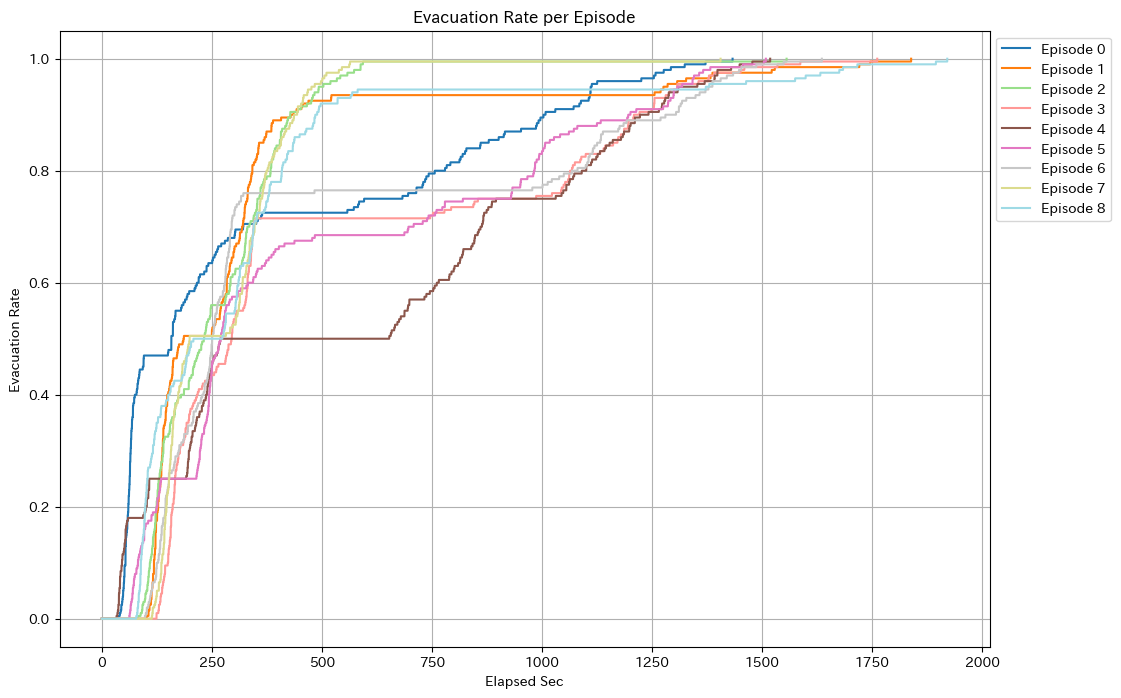
\includegraphics[width=\textwidth]{Figures/Yokosuka-EvaOnly-ERE.png} % 画像A
      \caption{(a).避難者のみで避難行動を行う場合}
      \label{fig:yokosuka-guid-graph-a}
  \end{minipage}
  \hfill % 隙間を調整
  % 上段右側
  \begin{minipage}{0.45\textwidth}
      \centering
      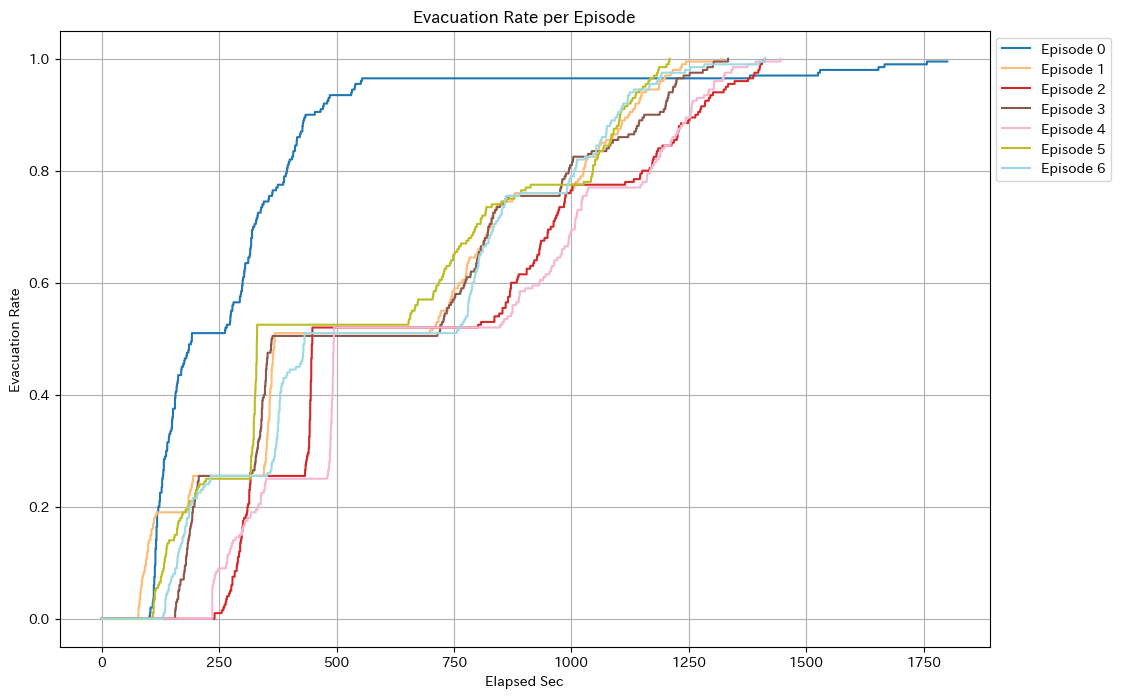
\includegraphics[width=\textwidth]{Figures/Yokosuka-RuleModel-ERE.png} % 画像B
      \caption{(b).ルールベースでの誘導の場合}
      \label{fig:yokosuka-guidgraph-b}
  \end{minipage}
  
  % 改行して下段中央
  \vspace{1em} % 適宜調整
  \begin{minipage}{0.65\textwidth}
      \centering
      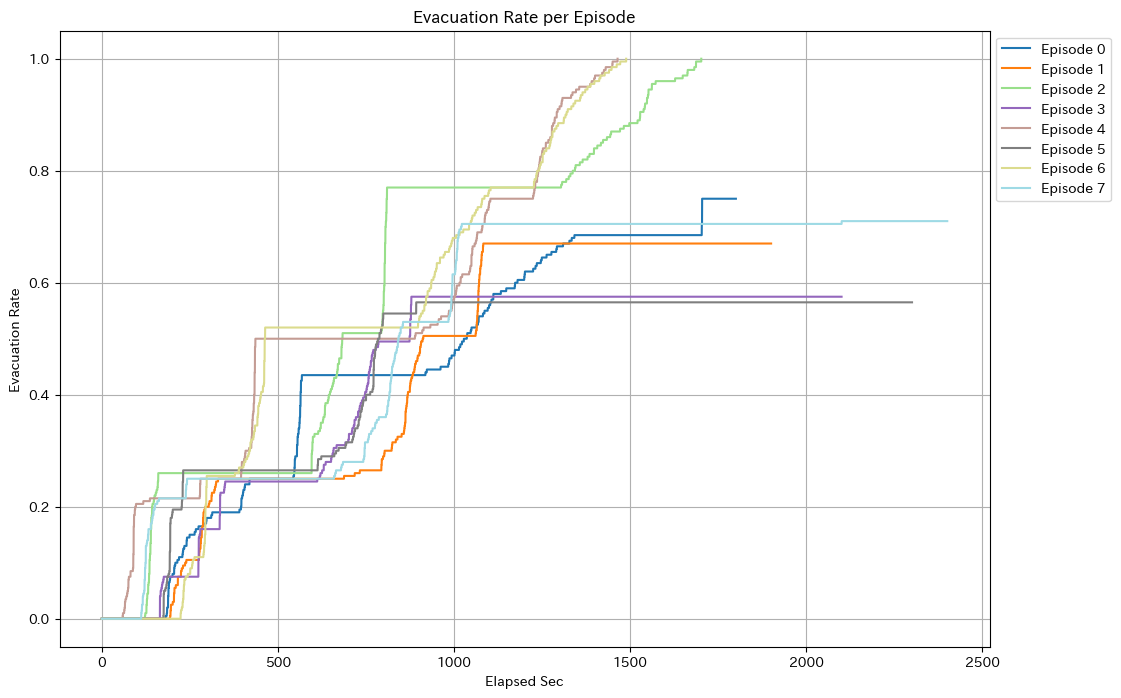
\includegraphics[width=\textwidth]{Figures/Yokosuka-AgentModel-ERE.png} % 画像C
      \caption{(c).学習済みマルチエージェントモデルによる誘導の場合}
      \label{fig:yokosuka-guidgraph-c}
  \end{minipage}
\end{figure}
横須賀市における環境においては,(c)マルチエージェントモデルによる誘導よりも,(b)ルールベースまたは(a)避難者のみで避難行動を行う場合の方が避難完了率の変化が速く,多くのエピソードにおいて最終的な避難完了率が$90\%$を超えており,高いことがわかる.
マルチエージェントモデルによる誘導では,多くの場合で避難完了率が60\%から70\%程度で収束しており,多くのケースで避難者全員を制限時間以内に避難所まで誘導することを達成出来なかった.
また,ルールベースと避難者のみでの結果のグラフに着目すると,避難者のみで行動する場合は,避難率が100\%になるまでに要した時間が1500秒前後なのに対し,ルールベースでの誘導を導入した場合は1250秒前後と,出現した避難者全員が避難完了するまでの時間が数分程度短縮されていることがわかる.\par

\subsubsection{沼津市のケース}
シミュレーション制限時間は240秒から1800秒の間で,エピソード毎に100秒ずつ増加する形で検証した.
以下に,沼津市のケースにおいて,各ケース毎に複数回シミュレートした結果の経過時間ごとの避難完了率の推移を示す.横軸がシミュレーション経過時間(秒)であり,縦軸が避難完了率である.
\begin{figure}[H]
  \centering
  % 上段左側
  \begin{minipage}{0.45\textwidth}
      \centering
      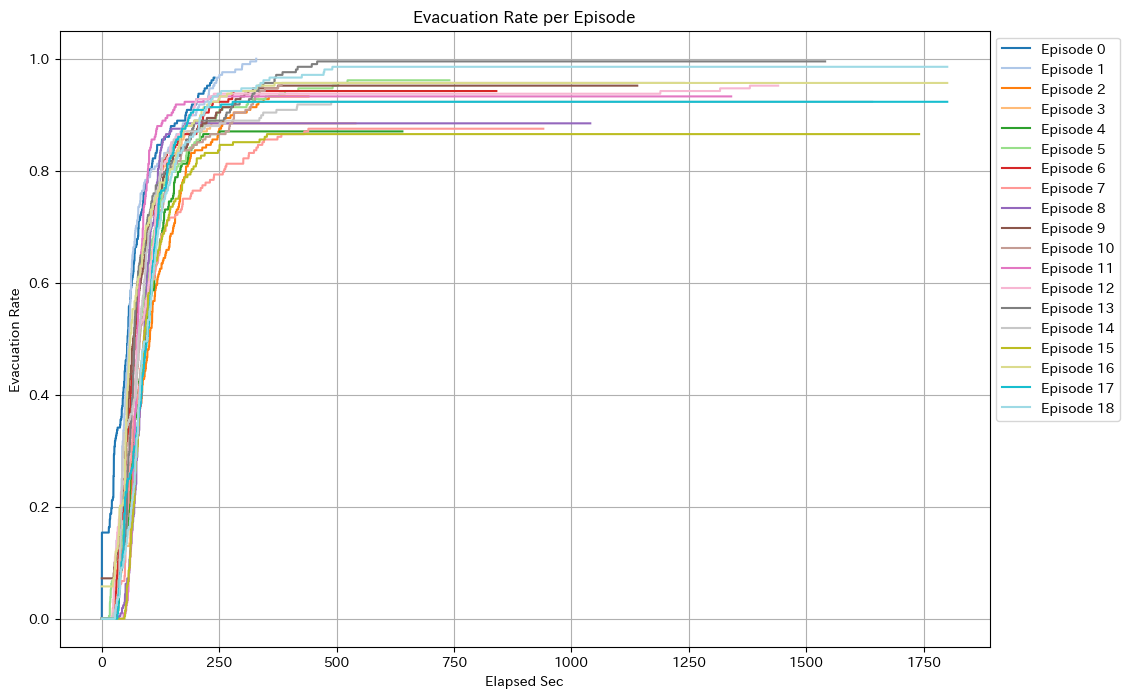
\includegraphics[width=\textwidth]{Figures/Numazu-EvaOnly-ERE.png} % 画像A
      \caption{(a).避難者のみで避難行動を行う場合}
      \label{fig:numazu-guid-graph-a}
  \end{minipage}
  \hfill % 隙間を調整
  % 上段右側
  \begin{minipage}{0.45\textwidth}
      \centering
      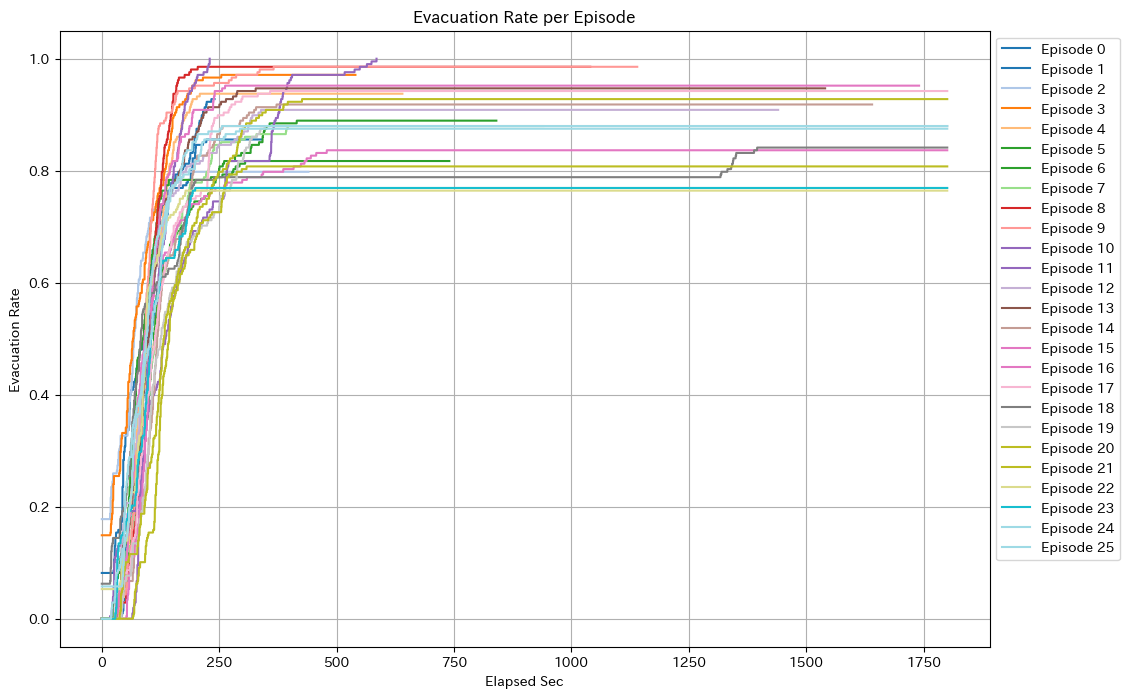
\includegraphics[width=\textwidth]{Figures/Numazu-RuleModel-ERE.png} % 画像B
      \caption{(b).ルールベースでの誘導の場合}
      \label{fig:numazu-guid-graph-b}
  \end{minipage}
  
  % 改行して下段中央
  \vspace{1em} % 適宜調整
  \begin{minipage}{0.65\textwidth}
      \centering
      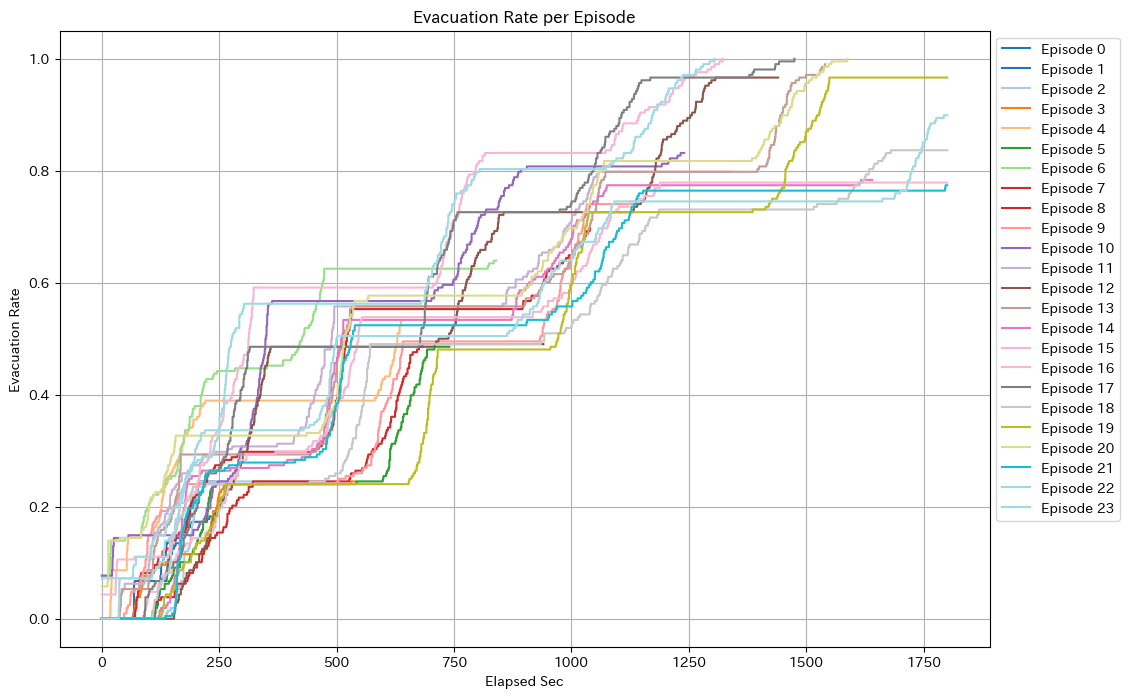
\includegraphics[width=\textwidth]{Figures/Numazu-AgentModel-ERE.png} % 画像C
      \caption{(c).学習済みマルチエージェントモデルによる誘導の場合}
      \label{fig:numazu-guid-graph-c}
  \end{minipage}
\end{figure}
沼津市のケースでは,(a)避難者のみで避難行動を行う場合と(b)ルールベースでの誘導を導入時の避難完了率の推移に大きな差は見られず,
どちらのケースも多くのエピソードで、短時間で避難完了率が90\%以上に達しており、全体的に迅速な避難が実現されている。
避難者のみで行動を行う場合,避難完了率が90\%を超えるまで開始から250秒以上経過してからが多いが,ルールベースでの誘導時は若干ではあるが250秒以下で避難完了率90\%を達成しているケースが多く,前者よりも避難完了率の上昇が早いことがわかる.
一方で,学習済みマルチエージェントモデルによる誘導時の避難完了率の推移を見ると,避難者のみで避難行動を行う場合やルールベースでの誘導を導入時と比較して,避難完了率の上昇が遅いことがわかる.
制限時間が短いエピソードでは避難完了率が20\%から40\%程に留まっている他,避難完了率が90\%を超えるまでに1200秒以上必要なエピソードが多く見られ,他のケースと比較して遅い避難完了率の推移が見られる.

\subsection{実験結果の考察}
避難所誘導タスクにおいて,図4.2から図4.7の結果から今回訓練したマルチエージェントモデルでは,多くの場合において避難完了率が90\%を超えることができず,避難者全員を制限時間内に避難所まで誘導することが難しいことがわかった.
また,経過時間あたりの避難完了率の伸び率からも,ルールベースでの誘導や避難者のみでの避難行動を行う場合と比較して,今回作成したマルチエージェントモデルによる誘導の方が遅いことが示された.
これは,図4.1の学習結果からもわかるように,モデルの学習が不十分であることが原因であると考えられる.
訓練全体を通じて,高い避難完了率を達成できるような方策をエージェントが経験できず,誘導人数や現在位置、避難所の収容人数に基づいた適切な誘導先の避難所を選択できなかったと考えられる.
また,モデルの予測精度を評価する指標の価値関数の平均損失の値が非常に高いことから,モデルの予測精度も低いことが言え,エージェントが報酬を最大化する適切な行動を出力できないということが言えるだろう.加えて,損失関数の減少が収束していないことからも,モデルの学習が不十分であると思われる.
これらは,訓練時間の不足や,ニューラルネットワークのハイパーパラメータの調整にまだ改善の余地があることを示しており,今後の課題として挙げられる.

また,エージェントの行動過程を観察分析すると,近隣の受け入れ可能な避難所を選択するのではなく、遠方の収容人数が多い避難所を選択する傾向が多く見られた.
このことが,他の方法と比較して遅い避難完了率の推移に繋がったと考えられる.
%TODO: その他推論時のエージェントの行動について動画を撮影し分析すること

沼津市の方が横須賀市よりも全体的な避難完了率が高いこと,経過推移が早いことが図\ref{fig:yokosuka-guid-graph-a}から図\ref{fig:numazu-guid-graph-c}の結果からわかる.
これは,沼津市の避難所配置が図\ref{fig:NumazuMap}のように\ref{fig:yokosukaMap}横須賀市よりも個数が多い他,対象範囲内にあまり位置に偏りなく避難所が配置されていることが影響していると考えられる.
横須賀市の場合は、対象範囲の両端それぞれに2か所の避難所が設けられているが,沼津市の場合は,横須賀市ほど避難所の配置は偏っておらず,その配置は放射状に配置されている他,近距離に他の避難所があるといった特性がある.
この様な都市ごとの環境的要因から1棟あたりの収容人数が横須賀市よりも少なく設定されているのにも関わらず,避難者が直ぐに近隣の避難所までたどり着けた傾向があり,全体的な避難完了率が横須賀市よりも高い結果となったと考えられる.
\begin{figure}[H]
  \centering
  % 1枚目の画像
  \begin{subfigure}{0.45\textwidth}
      \centering
      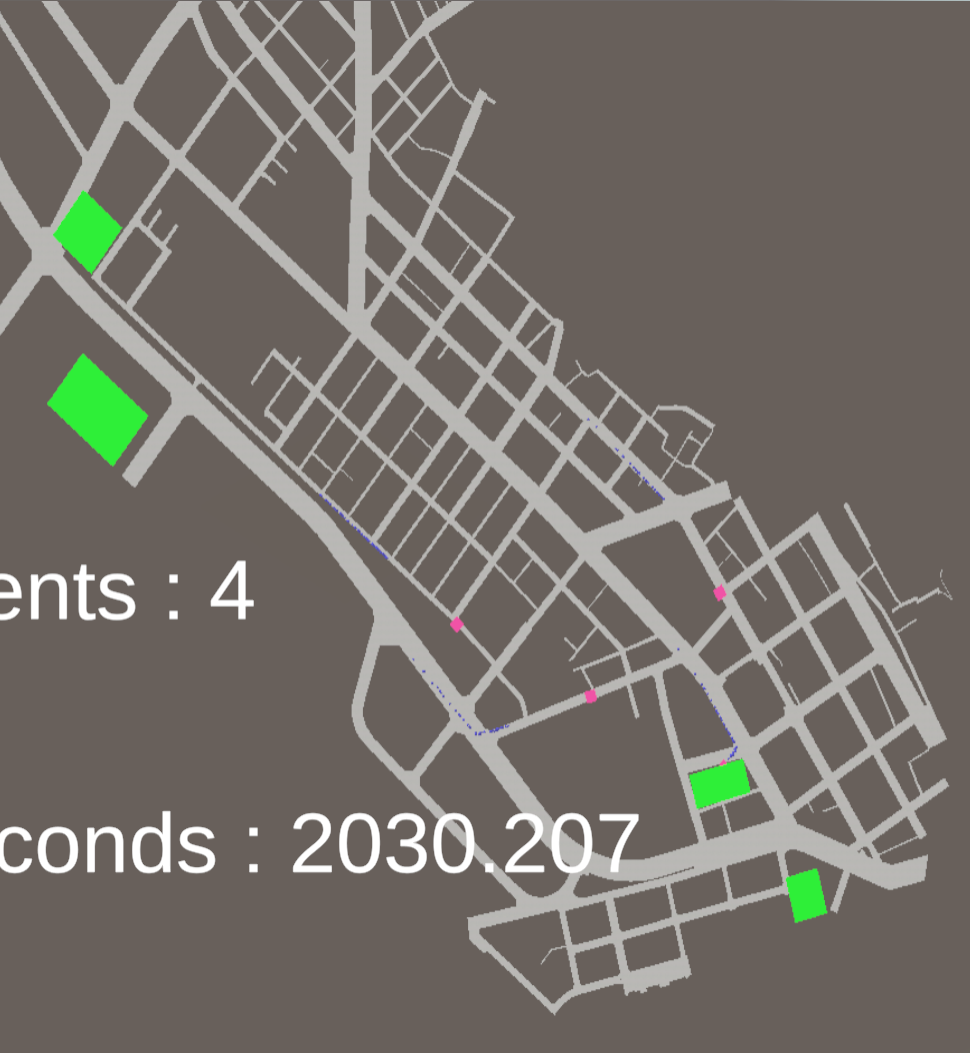
\includegraphics[width=0.85\textwidth]{Figures/Yokosuka-Map.png}
      \caption{横須賀市環境の全体図}
      \label{fig:yokosukaMap}
  \end{subfigure}
  % 2枚目の画像
  \begin{subfigure}{0.45\textwidth}
      \centering
      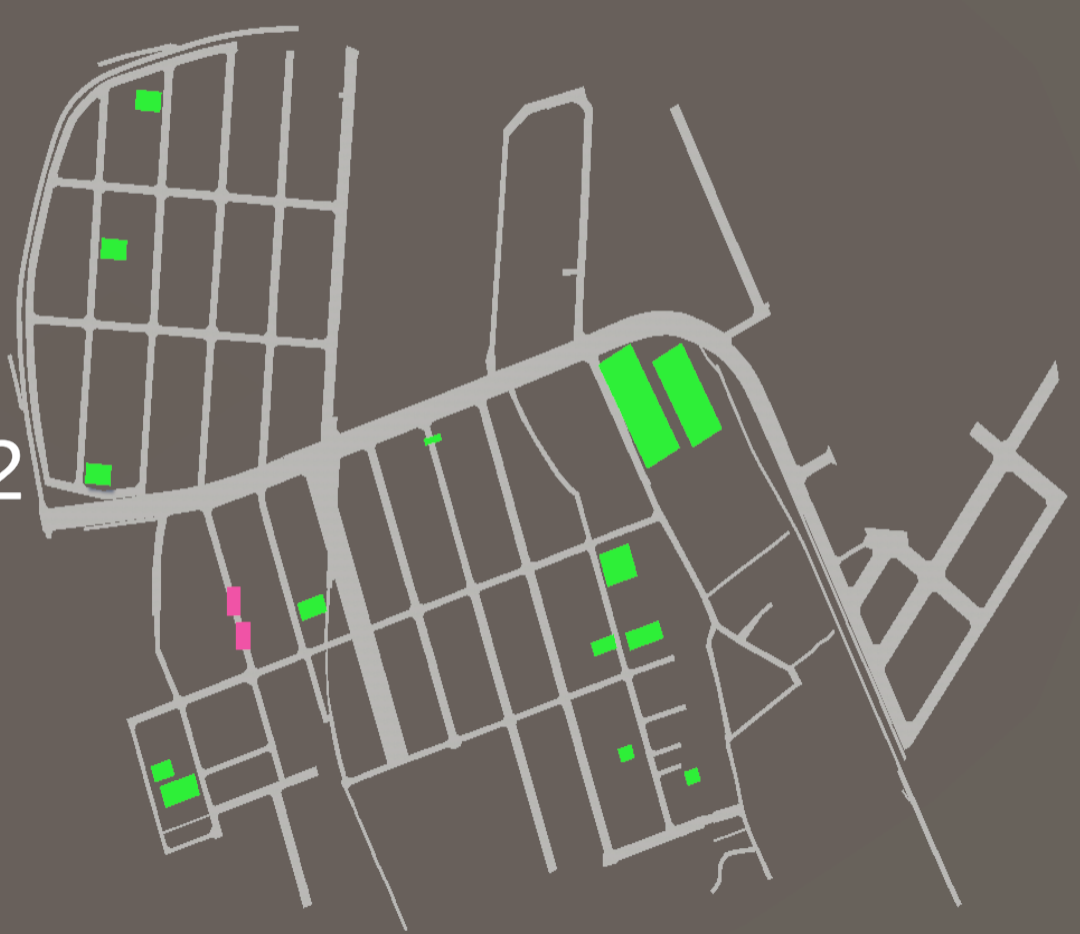
\includegraphics[width=\textwidth]{Figures/Numazu-Map.png}
      \caption{沼津市環境の全体図}
      \label{fig:NumazuMap}
  \end{subfigure}
  \caption{各都市の全体図(緑:避難所, 灰色:道路)}
  \label{fig:Maps}
\end{figure}